\begin{figure}[t]
\centering
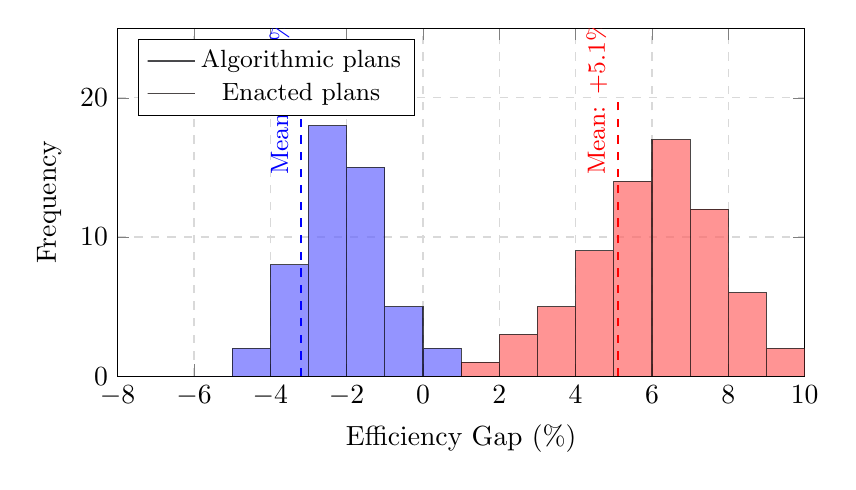
\begin{tikzpicture}
\begin{axis}[
    width=0.85\textwidth,
    height=6cm,
    xlabel={Efficiency Gap (\%)},
    ylabel={Frequency},
    ymin=0, ymax=25,
    xmin=-8, xmax=10,
    grid=major,
    legend pos=north west,
    legend style={font=\small},
    ymajorgrids=true,
    xmajorgrids=true,
    grid style={dashed,gray!30}
]

% Algorithmic plans distribution (centered around -3.2%)
\addplot[
    ybar interval,
    fill=blue!60,
    opacity=0.7,
    mark=none
] coordinates {
    (-6,0) (-5,2) (-4,8) (-3,18) (-2,15) (-1,5) (0,2) (1,0)
};
\addlegendentry{Algorithmic plans}

% Enacted plans distribution (centered around +5.1%)
\addplot[
    ybar interval,
    fill=red!60,
    opacity=0.7,
    mark=none
] coordinates {
    (0,0) (1,1) (2,3) (3,5) (4,9) (5,14) (6,17) (7,12) (8,6) (9,2) (10,1)
};
\addlegendentry{Enacted plans}

% Mean lines
\draw[blue, thick, dashed] (axis cs:-3.2,0) -- (axis cs:-3.2,20)
    node[above, rotate=90, anchor=south] {\small Mean: $-3.2\%$};

\draw[red, thick, dashed] (axis cs:5.1,0) -- (axis cs:5.1,20)
    node[above, rotate=90, anchor=south] {\small Mean: $+5.1\%$};

\end{axis}
\end{tikzpicture}

\caption{\textbf{Distribution of Efficiency Gaps: Algorithmic vs. Enacted Plans.}
Histogram showing the distribution of efficiency gaps across all competitive states and election years (N=45: 15 states $\times$ 3 years).
Algorithmic plans (blue) cluster around $-3.2\%$ Democratic advantage, while enacted plans (red) cluster around $+5.1\%$ Republican advantage.
The 8.3 percentage point separation demonstrates substantial partisan bias in enacted plans.
Dashed lines indicate mean values.}
\label{fig:eg-distribution}
\end{figure}
